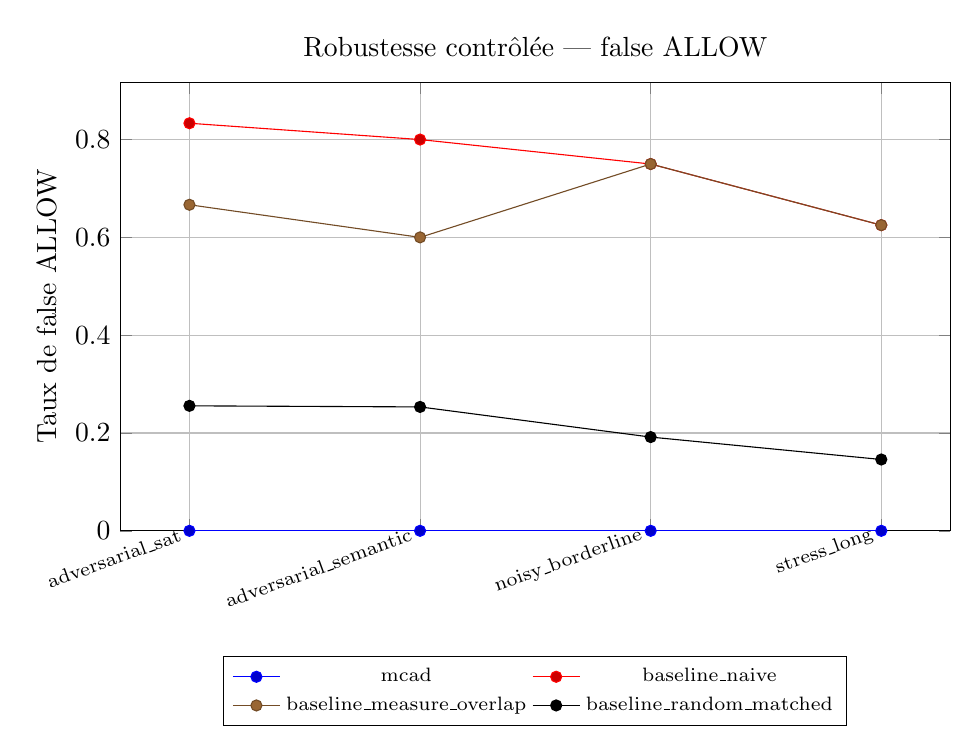
\begin{tikzpicture}
\begin{axis}[width=\linewidth,
height=0.60\linewidth,
title={Robustesse contrôlée — false ALLOW},
ylabel={Taux de false ALLOW},
xtick={0,1,2,3},
xticklabels={{adversarial\_sat},{adversarial\_semantic},{noisy\_borderline},{stress\_long}},
x tick label style={rotate=20,anchor=east,font=\scriptsize},
grid=major,
legend style={font=\scriptsize,at={(0.5,-0.28)},anchor=north,legend columns=2},
ymin=0]
\addplot+[mark=*] coordinates {(0,0.0) (1,0.0) (2,0.0) (3,0.0)};
\addlegendentry{mcad}
\addplot+[mark=*] coordinates {(0,0.833333) (1,0.8) (2,0.75) (3,0.625)};
\addlegendentry{baseline\_naive}
\addplot+[mark=*] coordinates {(0,0.666667) (1,0.6) (2,0.75) (3,0.625)};
\addlegendentry{baseline\_measure\_overlap}
\addplot+[mark=*] coordinates {(0,0.255556) (1,0.253333) (2,0.191667) (3,0.145833)};
\addlegendentry{baseline\_random\_matched}
\end{axis}
\end{tikzpicture}
